\documentclass[12pt]{article}

\usepackage{sbc-template}
\usepackage{graphicx,url}
\usepackage[utf8]{inputenc}
\usepackage{booktabs}
\usepackage{amsmath}

\renewcommand{\figurename}{Figura}
\renewcommand{\tablename}{Tabela}
\renewcommand{\refname}{Referências}

\sloppy

\title{O pré-treinamento clínico importa? Extração de relações de negação
em notas clínicas em português (RECLin-PT)}

\author{Angelo A. L. Silveira Filho\inst{1} \and Cristiano da Silveira
Colombo\inst{1}}

\address{Bacharelado em Sistemas de Informação\\
  Instituto Federal de Educação, Ciência e Tecnologia do Espírito Santo (IFES)\\
  Cachoeiro de Itapemirim -- ES -- Brasil
  \email{angeloalsf@gmail.com \quad cristiano.colombo@gmail.com}
}

\begin{document}

\maketitle

\begin{resumo}
O texto clínico livre concentra informação cuja interpretação depende da relação
entre conceitos, em especial a negação de achados. Como etapa inicial do
desenvolvimento do \textbf{RECLin-PT} --- modelo de extração de relações
(\emph{Relation Extraction}, RE) clínicas em português ---, este resumo apresenta
resultados preliminares de \emph{baselines}. Ajustamos dois \emph{encoders} sob
uma mesma infraestrutura experimental, um clínico (BioBERTpt) e um geral
(BERTimbau), sobre o corpus SemClinBr, em três classes (negação, associação e
ausência de relação), variando apenas o \emph{checkpoint} de pré-treino. No teste
congelado, os dois \emph{baselines} empatam estatisticamente no F1 de negação
(0,724 vs.\ 0,734; McNemar $p=0,18$; \emph{bootstrap} pareado IC95\%
$[-0,047;+0,026]$), e a variação entre sementes supera a diferença entre eles. O
RECLin-PT pode, portanto, ser construído sobre o \emph{encoder} geral, mais
eficiente, sem penalidade significativa.
\end{resumo}

\section{Introdução e objetivo}

O registro eletrônico em saúde concentra grande parte da informação clínica sob a
forma de texto livre, redigido em linguagem natural com abreviações
idiossincráticas e construções negativas características do discurso médico. Saber
que uma nota menciona ``febre'' não basta: é preciso distinguir se a febre está
\emph{associada} ao quadro do paciente ou se está sendo \emph{negada} (``paciente
afebril''). Esse vínculo é o objeto da extração de relações (RE), modelada aqui
como a classificação de um par ordenado de entidades $(e_1, e_2)$ no espaço de
rótulos \texttt{negation\_of}, \texttt{associated\_with} e \texttt{no\_relation}.
Tratar um achado negado como presente pode inverter por completo a interpretação
de um prontuário, o que torna a negação clínica um fenômeno de alto impacto.

Em português, a negação é fortemente lexicalizada (``não'', ``sem'', ``nega'',
``ausência de''), e há a expectativa difundida de que modelos pré-treinados em
texto do próprio domínio clínico capturem melhor essas construções do que modelos
de domínio geral. Essa expectativa, porém, é raramente testada de forma
controlada para o português. Este trabalho integra o desenvolvimento do
\textbf{RECLin-PT} e, como etapa inicial, responde a uma questão que fundamenta as
decisões de projeto seguintes: \textbf{o pré-treinamento clínico importa para a
extração de relações em textos médicos em português?} Comparam-se dois
\emph{encoders} sobre o SemClinBr~\cite{oliveira:22}, mudando \emph{somente} o
\emph{checkpoint} de pré-treino: o BioBERTpt~\cite{schneider:20}, adaptado a
narrativas clínicas em português, e o BERTimbau~\cite{souza:20}, de domínio geral.
O RECLin-PT será desenvolvido a partir do \emph{encoder} que se mostrar a melhor
base.

\section{Metodologia}

A premissa metodológica central é a \emph{paridade}: os dois \emph{baselines}
compartilham um único núcleo de implementação e diferem apenas no \emph{checkpoint}
de pré-treino, de modo que qualquer diferença observada seja atribuível ao
domínio do pré-treino, e não a artefatos. Toda a cadeia é determinística, com
semente fixa (42).

\noindent\textbf{Corpus e candidatos.} Usa-se o SemClinBr~\cite{oliveira:22}, com
1.000 documentos clínicos anotados (45.508 entidades; 11.458 relações, das quais
86,0\% \texttt{associated\_with} e 14,0\% \texttt{negation\_of}). Os dados são
particionados 80/10/10 em nível de \emph{documento} --- evitando vazamento ---,
com estratificação multirrótulo~\cite{sechidis:11}. Como o corpus anota apenas
relações positivas, geram-se pares candidatos percorrendo os pares ordenados
$(e_1,e_2)$ dentro de uma janela máxima (\texttt{max\_gap}$=20$); pares não
anotados recebem \texttt{no\_relation}. O resultado é um teste com 16.074 pares
(14.959 \texttt{no\_relation}, 964 \texttt{associated\_with}, 151
\texttt{negation\_of}).

\noindent\textbf{Representação e modelos.} Cada par vira a entrada
\texttt{[E1] <grupo>:\,superfície [/E1] $\ldots$ [E2] <grupo>:\,superfície [/E2]},
com marcadores tipados~\cite{soares:19}; os tipos UMLS são agregados nos 15 grupos
semânticos~\cite{mccray:01}, acrescidos das camadas \texttt{Abbreviation} e
\texttt{Negation}. Comparam-se o \textbf{BioBERTpt} (\emph{clínico}; 177,9~M
parâmetros) e o \textbf{BERTimbau} (\emph{geral}; 108,9~M), ambos com perda de
entropia cruzada \texttt{balanced}, escalonador linear com \emph{warmup}, seleção
por macro-F1 no desenvolvimento e mesmos hiperparâmetros. A métrica principal é o
macro-F1; a comparação usa o teste de McNemar~\cite{dietterich:98} e um
\emph{bootstrap} pareado (10.000 reamostragens) no F1 de \texttt{negation\_of}.

\section{Resultados preliminares}

Os dois \emph{baselines} apresentam desempenho praticamente indistinguível
(Tabela~\ref{tab:res}). O BioBERTpt clínico atinge macro-F1 de 0,707 e o BERTimbau
geral, 0,704. Na métrica-alvo, o F1 de \texttt{negation\_of}, a ordem inclusive se
inverte: o BERTimbau geral (0,734) supera marginalmente o BioBERTpt clínico
(0,724). Ambos alcançam \emph{recall} alto na negação ($\approx$0,89) e têm em
\texttt{associated\_with} a maior dificuldade, refletindo a confusão entre
associação genuína e mera proximidade textual (Figura~\ref{fig:f1classe}).

\begin{table}[ht]
\centering
\caption{Resultados dos \emph{baselines} no teste (semente 42). Negrito indica o
melhor valor por coluna.}
\label{tab:res}
\begin{tabular}{lcccc}
\toprule
\textbf{Baseline} & \textbf{Macro-F1} & \textbf{F1 neg.} & \textbf{MCC} &
\textbf{Acur.} \\
\midrule
BioBERTpt (clínico) & \textbf{0,707} & 0,724 & \textbf{0,487} & \textbf{0,885} \\
BERTimbau (geral)   & 0,704 & \textbf{0,734} & 0,471 & 0,882 \\
\bottomrule
\end{tabular}
\end{table}

\begin{figure}[ht]
\centering
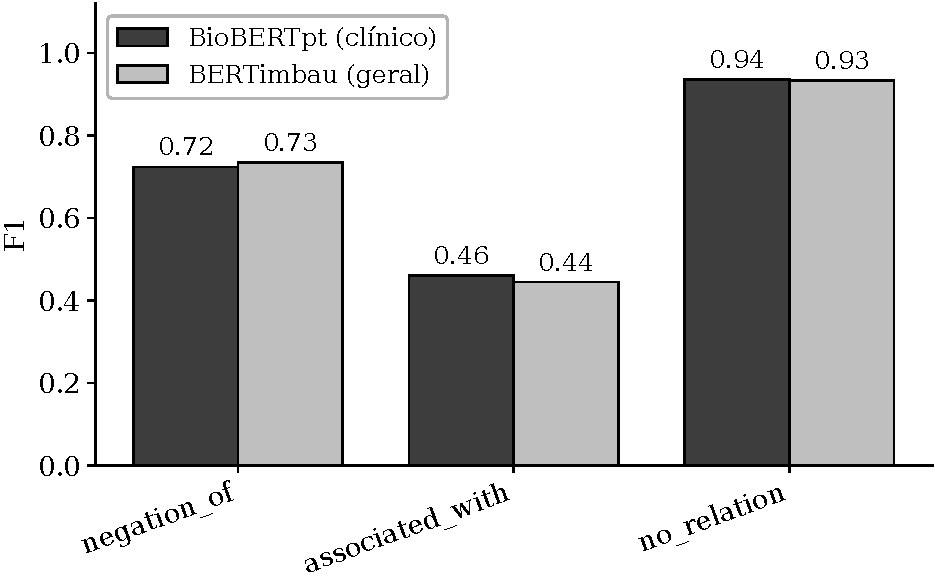
\includegraphics[width=.62\textwidth]{figs/f1_por_classe.pdf}
\caption{F1 por classe no teste: BioBERTpt (clínico) vs.\ BERTimbau (geral). As
barras são praticamente coincidentes em todas as classes.}
\label{fig:f1classe}
\end{figure}

\noindent\textbf{Significância.} A proximidade dos valores sugere empate, e o
teste pareado confirma. No F1 de \texttt{negation\_of}, a diferença observada é de
apenas $-0,010$ (a favor do BERTimbau). O McNemar não rejeita a igualdade
($p=0,18$): das 946 instâncias em que os modelos discordam, 494 favorecem o
BioBERTpt e 452 o BERTimbau. O \emph{bootstrap} pareado confirma: IC95\% de
$[-0,047;+0,026]$, que \emph{inclui o zero} (valor-$p=0,57$). Não há, portanto,
diferença estatisticamente significativa entre o \emph{encoder} clínico e o geral.

\noindent\textbf{Robustez à semente.} Treinando o BioBERTpt com uma segunda
semente (43), o F1 de \texttt{negation\_of} cai de 0,724 para 0,653 --- variação
de 0,071 atribuível \emph{apenas} à inicialização, cerca de sete vezes maior que a
diferença de 0,010 entre os dois modelos. O ruído de treino do próprio
\emph{encoder} clínico supera a vantagem que se poderia atribuir ao domínio de
pré-treino, reforçando a leitura de empate.

\section{Considerações parciais}

O resultado central é um \emph{empate estatístico}: para a RE no SemClinBr, em
três classes, o pré-treinamento clínico não produz vantagem mensurável sobre o
geral, nem mesmo na negação. Isso é plausível porque a negação em português é
altamente lexicalizada --- acessível também a um \emph{encoder} geral --- e porque
a tarefa depende mais da estrutura local do par (direção, proximidade, tipos
semânticos) do que de conhecimento lexical especializado, estrutura fornecida
igualmente aos dois modelos pela representação de entrada. Um corolário prático é
a eficiência: o BERTimbau iguala o BioBERTpt com $\approx$60\% dos parâmetros.

Esses resultados preliminares orientam a próxima etapa: o RECLin-PT será
construído sobre o \emph{encoder} geral, mais eficiente, com foco no aprimoramento
da classe \texttt{negation\_of}, a mais crítica para a interpretação clínica. Como
próximos passos, prevê-se estimar os \emph{baselines} sob múltiplas sementes,
estender o espaço de relações para além das três classes e integrar uma etapa de
NER automática para avaliar a RE em um cenário fim a fim.

\bibliographystyle{sbc}
\bibliography{artigo}

\end{document}
